\chapter{Future Work}
\label{ch:future}


\section{Anticipated TR WPT System}
\label{sec:future-roadmap}
\todo{Let's think of a better name!}

This research represents a first step in the exploration of building a
time reversal WPT system.
%
We demonstrate one possible realization of this idea in Fig.~\ref{fig:SysImage}.


The proposed system consists of two basic components.
%
The first is a rectenna that serves as the receiver.
%
The system as described in Section~\ref{sec:ltr-meth} would require an
out-of-band feedback channel between the receiver and transmitter. However, we
have demonstrated in Section~\ref{sec:selective-sim} that a transmitter can target
receivers entirely in-band.
%
Our system in Fig.~\ref{fig:SysImage} builds on these findings.
%
The second is a transmitter that performs the time reversal process.
%
This component is responsible for recording characteristic signals from the
receiver(s), time reversing the signals, and re-broadcasting them into the
environment.



In a practical system, the rectenna will be integrated into the hardware of a
mobile device, or into an external component that plugs into the battery.
%
The transmitter would  be connected to an external power source, but
could otherwise be located anywhere in the room.

Although not a component of the system, another important consideration in this
scenario is the environment; a low-loss scattering environment is necessary for
time reversal to be effective.

\begin{figure}[t]
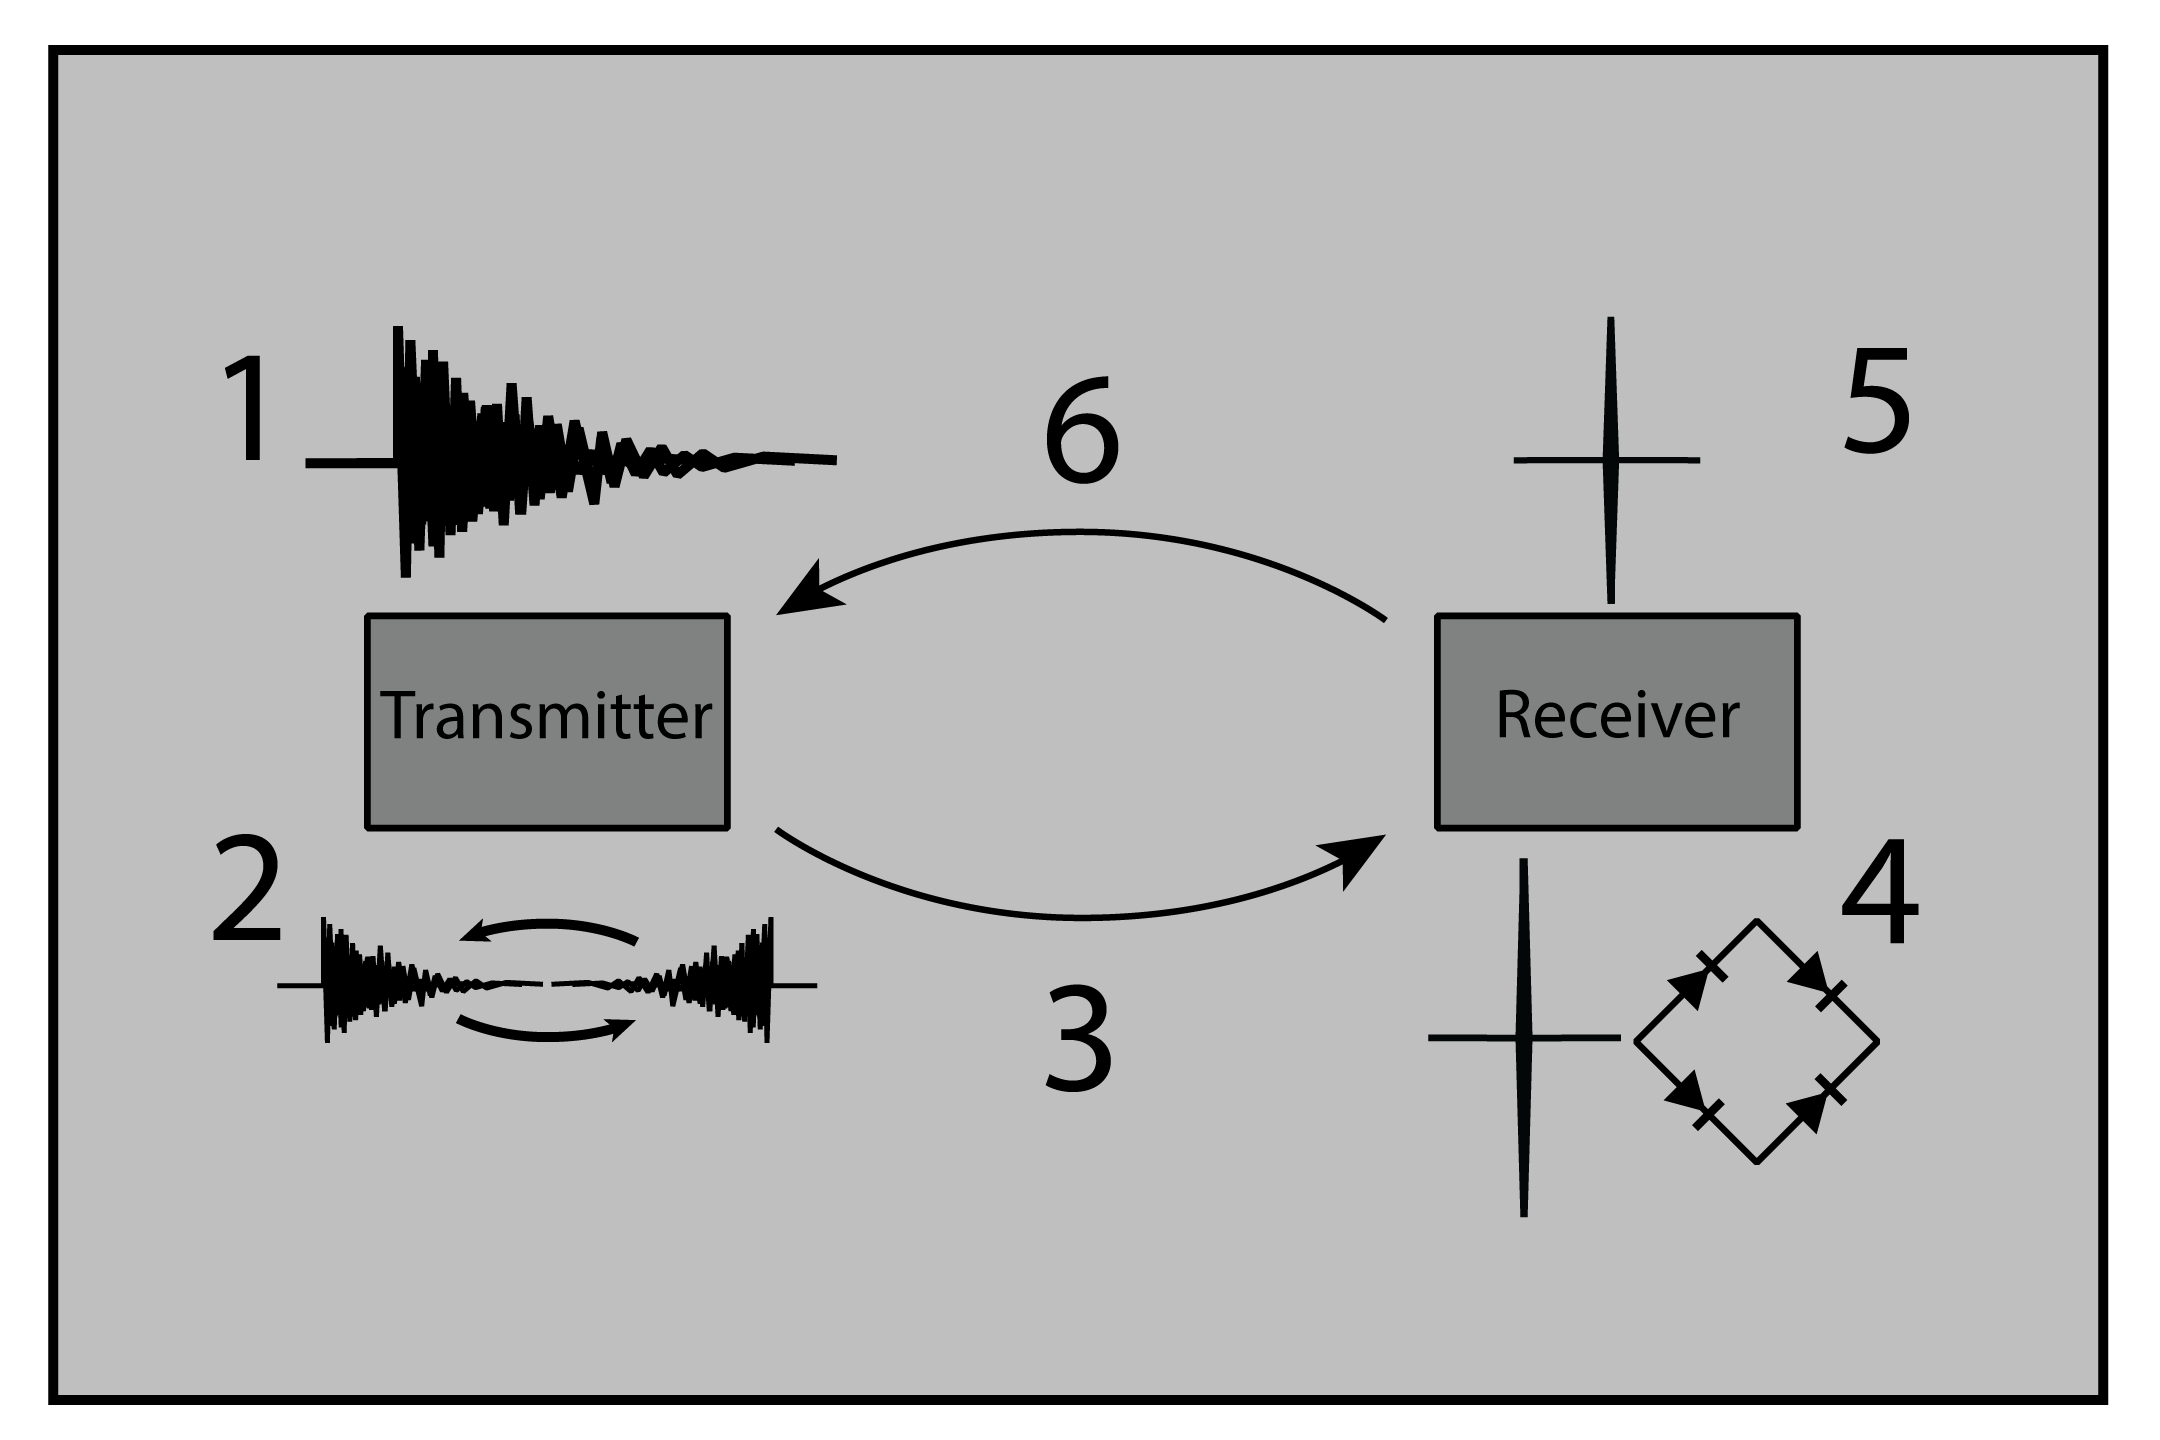
\includegraphics[width=\columnwidth]{figs/future/WPTSys}
\caption{A notional time reversal WPT system. In the acquistion phase, a new receiver joins the system by broadcasting or emitting a characteristic signal (0). Here, the receiver actively emits a signal, but it is also possible for the transmitter to find a passive target, as shown in~\cite{nltr-wave-chaotic}. In either case, the next sona that the transmitter collects will contain spatial information unique to the receiver's location (1). In the power transfer cycle, the sona is time reversed (2), amplified, and broadcast back into the environment. The amplified signal reconstructs on the receiver (3) and is converted to usable DC power by the rectifier (4). A small fraction of the signal is used to re-broadcast a new characteristic signal (5) into the environment, which will be collected in the next sona (6). The cycle repeats from (2).}
\label{fig:SysImage}
\end{figure}

We have demonstrated the underlying concepts of the WPT system depicted in Fig.~\ref{fig:SysImage}.
However, much work is necessary to transform this proof-of-concept technology to a functional product that consumers may use.
Future work discussed here falls into one of two categories. The first category includes established TR techniques that may be extended into the field of TR WPT.
The second category includes novel designs proposed by the team applicable only to TR WPT. Both will be discussed below. 

\section{Future work on applying other techniques from TR to WPT}
\label{sec:future-tr}
\todo{Is this redundant with the intro? Also, kinda awkward, but I can't think of anything better}
Imaging of objects and non-invasive surgery have been major applications of TR in the past.
As a result  many techniques have been developed to improve reconstruction quality on a target.
We suspect that many of these techniques may have applicability to our proposed system, but did not
have the opportunity to investigate them in our research.
However, stationary TR methods have different design priorities than our proposed TR WPT system.
These differences are significant enough that we suggest that dedicated experiments for WPT applicability may be useful.

\subsection{Iterations}

It has been well proven in the literature that time reversal focusing on an object can be repeated to improve
waveform collapse on a target. \todo{cite a fink acoustic paper showing this} \todo{We need to define what ``improved waveform collapse'' is} However, this technique has not been applied to TR WPT.

We suspect that applying iterative TR can "prune" reflection orbits that contribute poorly to the final reconstruction, in favor of ones that do. We predict that we can maximize our efficiency and reconstruction quality using this method. Additionally, we predict that this method will only be useful for stationary targets.

Both of these characteristics can be easily tested, using algorithms already applied to acoustic TR. An experimental setup very similar to ours could be applied to this research. A faster refresh rate \todo{Is refresh rate the correct term?} would be required from the TR system for this method to be able to outpace the natural ``decay'' of the testing environment. Once an iterative algorithm has been tested and found successful it should be tested in a less homogeneously reflective environment, to determine if it can be used to improve efficiency in lossy environments.

The novelty of such research is primarily in the characteristics measured. The demonstration (or not) of filtering of lossy paths would also be a major finding. Models should be generated relating the refresh rate \todo{see above comment about refresh rate} to performance gains using iterative method. If possible, multiple environments should be tested to generalize these results.

\subsection{Multiple Transmitters}

Many TR applications make use of multiple transmitters as a method of improving signal quality. Time reversal with multiple transmitters has the effect of improving the reconstruction strength at a target point. \todo{This statement is based off of a comment by Dr. Anlage. Need to verify/cite} All research done by the team was done using a single transmitting antenna. The incorporation of multiple antennas would require major modifications to our experimental setup, and was beyond our operating budget.

While final signal strength of the reconstruction is gauranteed to increase, how much remains to be determined. Future research should attempt to determine how multiple antennas relate to the efficiency of transfer. Particular attention to how this efficiency changes as sources of loss are introduced into the system.

\subsection{Expontential Amplification}

\todo{Currently reading this in Bini's paper.}

Basic idea is that we know that exponential amplification can be used to counteract losses generated by the system. Exponential sona amplification is a nonlinear amplification to the sona across its timespan. It is meant to counteract the larger losses (due to larger number of reflections) experienced by reflective orbits with larger paths. This technique has been shown to increase the efficacy of the recontstructed waveform, by decreasing additional signal delivered to the receiver.

However, it should be understood that this is a method for compensating for the losses experienced by a time reversed signal. It does not remove these losses, and in face more energy is lost through this method. As a result, effiency using this method decreases. This introduces a tradeoff to using the method that could be significant to designers of a TR WPT system. Experiments should focus on quantifying the aspects of this tradeoff so that informed decisions can be made in the design of future systems.

\section{New problems that arise with TR in a WPT context}
\label{sec:future-wpt}

There are additional challenges involved with a TR WPT sytem that create avenues for research and innovation. Many of these deal with addressing the differing design goals with a TR WPT system - most TR applications care little about efficiency, caring only about the fidelity of the reconstruction on the target. In TR WPT the opposite is true - perfect reconstructions are far less important than the efficiency of transfer.

Most TR applications consider stationary - or near stationary - targets. TR WPT system must always consider moving targets. We have demonstrated that rapid recollection of sonas can compensate for the loss of 

Additionally, the demand for optimal efficiency requires TR WPT to consider the characteristics of the environment moreso than ordinary TR applications.

\subsection{Sub Cavity}

Stuff

\subsection{That other thing}

Stuff

\subsection{Timing Analysis}

Stuff

\subsection{Rectenna Design}
